%%%%%%%%%%%%%%%%%%%%%%%%%%%%%%%%%%%%%%%%%%%%%%%%%%%%%%%%%%%%%%%%%%%%%%%%%%%%%%%%%%%%%%%%%%
%%%%%%%This is the code to generate the User Manual for the fMRI Design Explorer %%%%%%%%%
%%%%%%%%%%%%%%%%%%%%%%%%%%%% Author: Dustin Moraczewski %%%%%%%%%%%%%%%%%%%%%%%%%%%%%%%%%%
%%%%%%%%%%%%%%%%%%%%%%%%%%%%%%%%%%%%%%%%%%%%%%%%%%%%%%%%%%%%%%%%%%%%%%%%%%%%%%%%%%%%%%%%%%

%%%%%%%%%% Import Packages %%%%%%%%%%
\documentclass[10pt]{article}
\usepackage[margin=1in,headheight=15pt]{geometry}
\usepackage[scaled]{helvet}
\usepackage[utf8]{inputenc}
\usepackage[english]{babel}
\usepackage[english]{isodate}
\usepackage[parfill]{parskip}
\usepackage[notocbib]{apacite}
\usepackage{hyperref,listings}
\usepackage{titlesec,fancyhdr}
\usepackage{graphicx,subcaption,wrapfig}
\usepackage[usenames,dvipsnames]{xcolor}
\usepackage[export]{adjustbox}
\usepackage{tikz,tikz-qtree}
\usepackage{environ,textcomp,amssymb}

%%%%%%%%%% Set up %%%%%%%%%%
% fancy header stuff
\pagestyle{fancy}
\fancyhf{}
\renewcommand{\headrulewidth}{0pt}
% set up hyper link format
\hypersetup{
	pdfauthor={Dustin Moraczewski},
	pdfcreator={Dustin Moraczewski},
	colorlinks=true,
	}
% set up code display format
\lstset{
	keywordstyle=\color{blue},
	basicstyle=\ttfamily,
	commentstyle={},
	columns=flexible,
	showstringspaces=false,
	keepspaces=True,
	upquote=True,
	belowskip=0mm,
	}
% define command for a typical tab space
\newcommand\tab[1][1cm]{\hspace*{#1}}
% define spacing for sections, subsections, and subsubsections
\titlespacing*{\section}{0mm}{0mm}{4mm}
\titlespacing*{\subsection}{0mm}{4mm}{0mm}
\titlespacing*{\subsubsection}{0mm}{2mm}{0mm}
% define environment for hierarchy flow charts
\makeatletter
\newsavebox{\measure@tikzpicture}
\NewEnviron{scaletikzpicturetowidth}[1]{%
  \def\tikz@width{#1}%
  \def\tikzscale{1}\begin{lrbox}{\measure@tikzpicture}%
  \BODY
  \end{lrbox}%
  \pgfmathparse{#1/\wd\measure@tikzpicture}%
  \edef\tikzscale{\pgfmathresult}%
  \BODY
}
\makeatother
\newcommand*\circled[1]{\tikz[baseline=(char.base)]{
            \node[shape=circle,draw,inner sep=.5pt] (char) {#1};}}
% define section and subsection headings and format
\renewcommand{\thesection}{}
\renewcommand{\thesubsection}{\arabic{section}.\arabic{subsection}}
\makeatletter
\def\@seccntformat#1{\csname #1ignore\expandafter\endcsname\csname the#1\endcsname\quad}
\let\sectionignore\@gobbletwo
\let\latex@numberline\numberline
\def\numberline#1{\if\relax#1\relax\else\latex@numberline{#1}\fi}
\makeatother
% create button micro-figures
% help
\newcommand*{\hbut}{
\includegraphics[scale=0.45]{fig/0_help.jpg}}
% new
\newcommand*{\nbut}{
\includegraphics[scale=0.02]{fig/0_new.png}}

%%%%%%%%%%%%%%%%%%%%%%%%%%%%%%
%%%%%%%%%% Document %%%%%%%%%%
%%%%%%%%%%%%%%%%%%%%%%%%%%%%%%

\begin{document}
% set tikz environment for flow charts / hierarchy
\tikzset{edge from parent/.style=
{draw, edge from parent path={(\tikzparentnode.south)
-- +(0,-8pt)
-| (\tikzchildnode)}},
blank/.style={draw=none},
level distance=35pt}

%%%%%%%%%% Title %%%%%%%%%%
\begin{titlepage}
	\vspace*{\fill}
	\begin{center}
		\Huge{fMRI Design Explorer:} \\
		\vspace{3mm}
		\LARGE{A program to design, optimize, and visualize task-based fMRI experimental designs} \\
		\vspace{10mm}
		\LARGE{User Manual} \\
		\vspace*{\fill}
		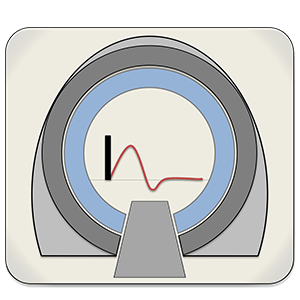
\includegraphics[width=.3\textwidth]{fig/de_icon.png}
	\end{center}
	\vspace*{\fill}
	\flushright{version 2016-10-27.1709}
\end{titlepage}
\newpage

%%%%%%%%%%%%%%%%%%%%%%%%%%%%%%%%%%%%%%%
%%%%%%%%%% Table of Contents %%%%%%%%%%
%%%%%%%%%%%%%%%%%%%%%%%%%%%%%%%%%%%%%%%
\hypersetup{
	linkcolor=black,
	}
\pagenumbering{Roman}
\tableofcontents
\label{sec:toc}
\newpage
\listoffigures
% \newpage
% \listoftables
\newpage

%%%%%%%%%%%%%%%%%%%%%%%%%%%%%%%%%%
%%%%%%%%%% Introduction %%%%%%%%%%
%%%%%%%%%%%%%%%%%%%%%%%%%%%%%%%%%%
% change link colors
\hypersetup{
	linkcolor=PineGreen,
	urlcolor=RoyalBlue,
	}
% numbers not numerals
\pagenumbering{arabic}
% header and footer stuff
\renewcommand{\footrulewidth}{0.5pt}
\rhead{\vspace*{\fill} Page \thepage}
\cfoot{\vspace*{\fill}\href{https://en.wikipedia.org/wiki/Haemodynamic_response}{
\includegraphics[scale=0.1]{fig/hrf.jpg}}}
% now begin...
\section{Introduction}
\label{sec:into}
	\textbf{Complete introduction forthcoming}

	\subsection{About the Program}
	\label{subsec:intro.prog}

	\subsection{About this Manual}
	\label{subsec:intro.manu}
		This manual provides an interactive and comprehensive description of the functionality of the fMRI Design Explorer.
		When this PDF is viewed electronically, it offers a number of helpful internal and external hyperlinks.
		In addition, hovering over the hyperlink with a mouse should result in a preview of the link's content.
		These hyperlinks have been tested on both Mac OS X and Linux operating systems.
		However, individual operating system and PDF viewer idiosyncrasies may prevent functional hyperlinks.
		Please report all hyperlink issues to Dustin Moraczewski at \href{mailto:dmoracze@umd.edu}{dmoracze@umd.edu}.

		\subsubsection{Internal Hyperlinks}
		\label{subsubsec:internal}
			Hyperlinks colored \textcolor{PineGreen}{green} refer to internal links.
			Clicking an internal link will navigate the PDF to the corresponding section or figure.
			For example, if the text refers to \hyperref[fig:launch]{Figure \ref{fig:launch}}, clicking on this link will navigate the PDF to Figure 1.
			In addition, the \hyperref[sec:toc]{Table of Contents} is fully interactive, however (as you probably noticed) the text color is not \textcolor{PineGreen}{green}.
			This decision was made for readability.

		\subsubsection{External Hyperlinks}
		\label{subsubsec:external}
			Hyperlinks colored \textcolor{RoyalBlue}{blue} refer to external links.
			Clinking an external link will initiate behavior external to the PDF.
			There are three types of external links:
			\begin{enumerate}
				\item URL link - this will open a browser and navigate to a specific URL.
				\item Email link - this will open an email client, if one is configured (currently does not work on the University of Maryland's GLUE network)
				\item Download link - this will download relevant files (e.g. the Design Explorer installer).
				This link may also open a browser that navigates to Dropbox on certain operating systems.
			\end{enumerate}
			For example, if the text refers to the \href{https://afni.nimh.nih.gov}{AFNI} package for fMRI analysis, clicking on the corresponding link will open a browser that navigates to the AFNI homepage.

	\subsection{Other Documentation}
	\label{subsec:intro.other}
\newpage

%%%%%%%%%%%%%%%%%%%%%%%%%%%%%%%%%%
%%%%%%%%%% Installation %%%%%%%%%%
%%%%%%%%%%%%%%%%%%%%%%%%%%%%%%%%%%
\section{Installation}
\label{sec:install}

	\subsection{System Requirements}
	\label{subsec:reqs}
		64-bit machines running Mac OS X \& Linux have been tested. \\
		It is likely that the program will run on others and may fail with some.

		Windows operating system is not supported.

		\subsubsection{Dependencies}
		\label{subsubsec:depend}
			Mac OS X -- \href{https://www.xquartz.org}{XQuartz} is required. \\
			Linux -- no dependencies.

	\subsection{Download}
	\label{subsec:dl}
		Please download the current Design Explorer installer \href{https://www.dropbox.com/s/mqvr5v7393eyorn/Install_DesignExplorer_2016-10-26.0958?dl=1}{here}.

	\subsection{Install}
	\label{subsec:install}
		\begin{enumerate}
			\item Open Terminal console.
			\item Navigate to the directory that contains the installer.
\begin{lstlisting}
> cd <path_to_installer>
\end{lstlisting}
			\item Change installer to executable, changing the version number appropriately.
\begin{lstlisting}
> chmod 755 Install_DesignExplorer_XXXX-XX-XX.XXXX
\end{lstlisting}
			\item Run the installer.
\begin{lstlisting}
> ./InstallDesignExplorer
\end{lstlisting}
			\item Pay attention to the output in the terminal.
			If there is an error, you should report this text to the developers.
			\item Once the installer is finished, an executable file called \texttt{DesignExplorer} will be deposited into your home (\texttt{\textasciitilde}) directory.
		\end{enumerate}

	\subsection{Run}
	\label{subsec:run}
		\begin{enumerate}
		\item To run the Design Explorer you can either double click on the \texttt{DesignExplorer} file OR you can run the program in the terminal:
\begin{lstlisting}
> ~/DesignExplorer
\end{lstlisting}
		\end{enumerate}

	The executable file \texttt{DesignExplorer} is a bash script that points to a \texttt{\textasciitilde/.DesignExplorer} hidden directory that contains a python distribution, all dependencies, \href{https://afni.nimh.nih.gov/pub/dist/doc/program_help/3dDeconvolve.html}{AFNI's 3dDeconvolve}, and the \hyperref[subsec:default]{default project}.

	\subsection{Uninstall}
	\label{ininstall}
		To uninstall the Design Explorer, simply open the terminal and type:
\begin{lstlisting}
> rm -rf ~/.DesignExplorer
\end{lstlisting}
		Be aware, though, that this will also delete the \hyperref[subsec:default]{default project} as well.

	\vfill
	Please email \href{mailto:dmoracze@umd.edu}{Dustin Moraczewski} with any issues related to installation.
	Be sure to be as descriptive as possible and provide your system configuration, what you did, and what was the output.
\newpage

%%%%%%%%%%%%%%%%%%%%%%%%%%%%%%
%%%%%%%%%% Overview %%%%%%%%%%
%%%%%%%%%%%%%%%%%%%%%%%%%%%%%%
\section{Overview}
\label{sec:overview}
	To see the forest rather than jumping right to the trees, this section gives users a quick overview of the multiple large-scale features of the Design Explorer.
	In addition, this section provides tips on \hyperref[subsec:start]{getting started}, \hyperref[subsec:general]{general information} and an \hyperref[subsec:overview]{overview of the interface}.

	\subsection{Getting Started}
	\label{subsec:start}
		Upon \hyperref[subsec:run]{executing} the Design Explorer, the Project Launcher window will appear:
		\vspace{3mm}
		\begin{figure}[ht]
		\centering
		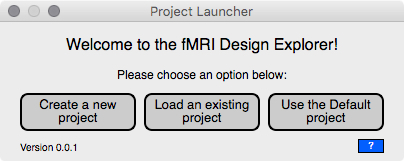
\includegraphics[width=0.4\textwidth,frame]{fig/1_launcher.jpg}
		\caption{Project Launcher}
		\label{fig:launch}
		\end{figure}

		Users have a three choices regarding how they want to initialize a project:
		\begin{enumerate}
			\item \hyperref[subsubsec:new]{Create a new project}
			\item \hyperref[subsubsec:load]{Load an existing project}
			\item \hyperref[subsec:default]{Use the Default  project}
		\end{enumerate}

		\subsubsection{Create a new project button}
		\label{subsubsec:new}
			To create a new project within a user-defined location, choose this option. 
			A file directory dialog window will appear and the user will need to choose a location for their new project.
			Typically, prior to the creation of a new project, users will create a unique directory for their project.
			This unique directory will ensure that all files relevant to the project are contained within a single location.
			\begin{enumerate}
				\item Choose the \textbf{Create a new project} button
				\item Navigate to desired directory
				\item Click \textbf{choose}
				\item Enter project name
				\item Click \textbf{ok}
			\end{enumerate}

			The new project will be created and the main window will appear (\hyperref[fig:overview]{Figure \ref{fig:overview}}).

		\subsubsection{Load an existing project button}
		\label{subsubsec:load}
			If a previous project had been created within a user-defined location (using the \hyperref[subsubsec:new]{Create a new project} button), users can choose to load this already existing project.
			\begin{enumerate}
				\item Choose the \textbf{Load an existing project button}
				\item Navigate to project's directory
				\item Click \textbf{choose}
			\end{enumerate}

			The project will load where the user left off, including all variants.

		\subsubsection{Use the Default project button}
		\label{subsec:default}
			The default project exists so that users can rapidly create and interact with experimental designs without cluttering up the file system.
			Upon initialization of the default project, the Design Explorer will deposit a directory called \texttt{default\_project} within the \texttt{\textasciitilde/.DesignExplorer} directory and the user will be asked to name the project.
			If a default project already exists, clicking the \textbf{Use the Default project} button will open the previously saved default project.

			To remove the default project, open a terminal and type:
\begin{lstlisting}
> rm -rf ~/.DesignExplorer/default_project
\end{lstlisting}

	\subsection{General Information}
	\label{subsec:general}

		\subsubsection{Autosave}
		\label{subsubsec:save}
			All changes within a valid design are autosaved, thus, there is no need to save manually.
			However, there is a caveat to the autosave feature: in order for changes to be saved, the changes must occur within a valid design and be valid with respect to the parameters of interest.
			For example, the autosave feature will not save changes under the following scenarios:
			\begin{enumerate}
				\item If events are defined and/or configured without first creating a design using the \nbut{} button, the changes will be lost because they did not occur within the context of a design.
				\item Entering a character instead of a number into the \textbf{TR} field would not be saved since this field expects a numeric value.
			\end{enumerate}

			These scenarios are meant to represent the types of behaviors that would fail to autosave and do \textbf{not} encompass all possibilities.

	\subsection{Overview of Interface}
	\label{subsec:overview}
		This section gives a brief overview of the main interface that is common to all Tabs.
		Please see the \hyperref[subsec:tabs]{Tabs} section for functionality unique to each Tab.
		\hyperref[fig:overview]{Figure \ref{fig:overview}} depicts the large-scale structure of the Design Explorer interface.
		\begin{figure}[ht]
			\centering
			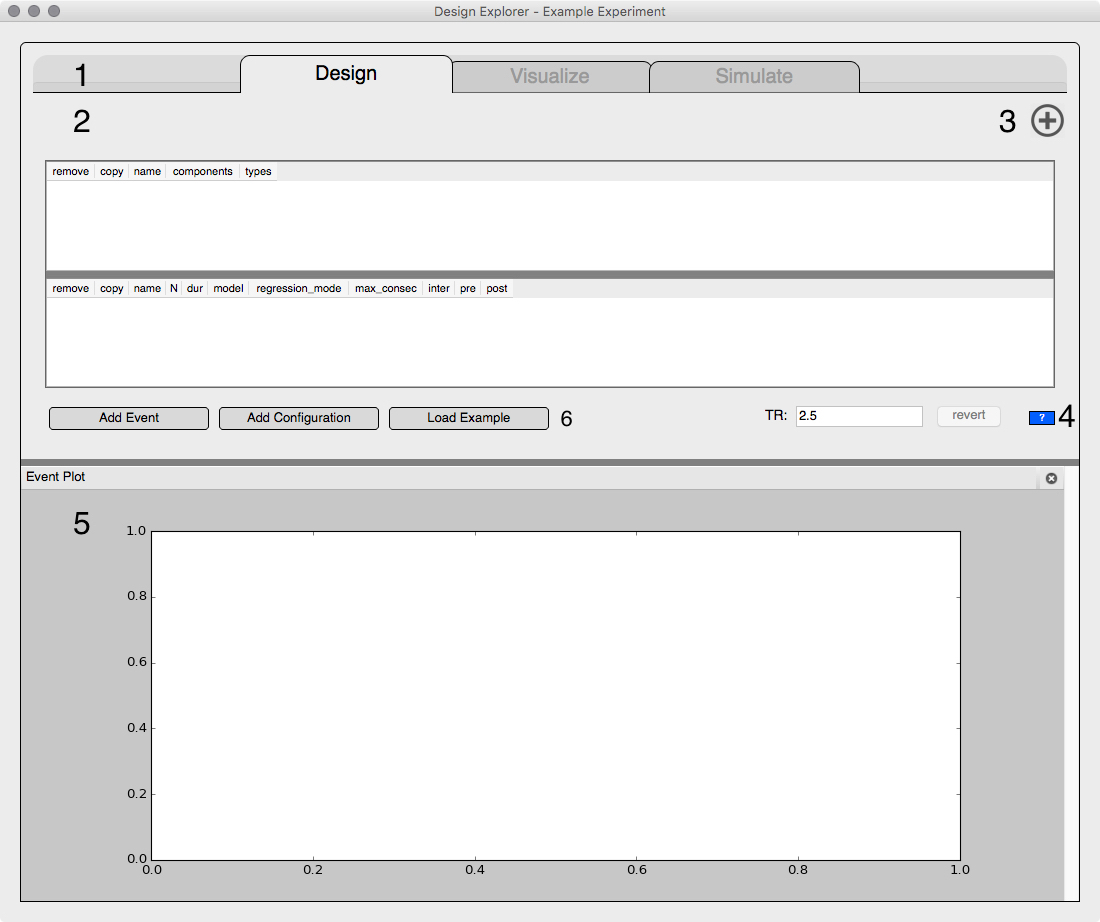
\includegraphics[width=0.75\textwidth,frame]{fig/2_overview.jpg}
			\caption{Overview of Interface}
			\label{fig:overview}
		\end{figure}

		Consider the number annotations in \hyperref[fig:overview]{Figure \ref{fig:overview}}:
		\begin{enumerate}
			\item The \hyperref[subsec:tabs]{Tab} menu: \\
			This menu consists of the main functional divisions of the Design Explorer.
			The tabs consist of \hyperref[subsubsec:design]{Design}, \hyperref[subsubsec:visualize]{Visualize}, and \hyperref[subsubsec:simulate]{Simulate}.
			\item The Design menu: \\
			This menu consists of the user-defined designs currently in the workspace.
			In \hyperref[fig:overview]{Figure \ref{fig:overview}}, this menu is currently blank which means that no designs have been created yet.
			A design must be created before defining or configuring events.
			\item The New Design button \nbut{}: \\
			This button adds a new design to the Design Menu.
			When this button is clicked, users will be asked to enter a name for the new design.
			All designs must have unique names.
			\item The \hyperref[subsubsec:hbut]{Help Button} \hbut{} \\
			This button is available in all three tabs.
			\item The Plot window: \\
			This window is available in all tabs, however, the information presented within this window is unique to each tab.
			For example, the plot window in the \hyperref[subsubsec:design]{design tab} shows the event plots whereas this window in the \hyperref[subsubsec:visualize]{visualize} and \hyperref[subsubsec:simulate]{simulate} tabs show the ideal and simulated BOLD signal, respectively.
			\item The \hyperref[subsubsec:example]{Load Example button}: \\
			Click this button to load specific examples from this workbook.    
		\end{enumerate}

	\subsection{Tabs}
	\label{subsec:tabs}
		This section gives a brief, big-picture overview of the functionality of each of the tabs. Please see the corresponding chapters for greater detail regarding the implementation of the features.

		\subsubsection{Design}
		\label{subsubsec:design}
			The purpose of the Design tab is three-fold:
			\begin{enumerate}
				\item Define events into an event hierarchy
				\item Configure the various parameters of the events
				\item View experimental design as an event plot
			\end{enumerate}

			There are multiple ways in which users can define their event hierarchy, see the Event Hierarchy chapter for more information.
			With regards to event configuration, users have complete control of most parameters: number of events, event duration, hemodynamic response models, maximum consecutive events of the same type, pre, inter, and post baseline periods.
			Both events convolved with a hemodynamic response and not are configurable.

		\subsubsection{Visualize}
		\label{subsubsec:visualize}
			The purpose of the visualize tab is to view the idealized (no noise added) BOLD signal on your experiment.
			Users can also view event-specific signal to examine the relative contributions of each event to the overall BOLD signal.
			This signal is derived from the events that are configured to include a hemodynamic response model.
			In addition, the Event Configuration table is also supplied so that users can make adjustments to the event parameters and see the changes in the BOLD signal in real time.

		\subsubsection{Simulate}
		\label{subsubsec:simulate}
			The purpose of the Simulate tab is to use an experimental design to simulate BOLD signal according to user-defined event-specific $\beta$ weights, event-specific noise, as well as global noise.
			Then, once new BOLD signal is simulated, users can examine the error in the recovered $\beta$ estimates.
			The number of simulations is a user-defined parameter.

	\subsection{Help}
	\label{subsec:help}
		\subsubsection{The Load Example Button}
		\label{subsubsec:example}
			The load example button is a quick and easy way to load the designs discussed in the units of the workbook.
			Thus, users can load an example quickly and begin interacting with the designs without spending time defining and configuring each individual event.

		\subsubsection{The Help Button}
		\label{subsubsec:hbut}
			The help button \hbut{}, as seen in the lower right corner of \hyperref[fig:launch]{Figure \ref{fig:launch}}, will open this user manual to provide further assistance on the implications of these decisions.
			This button is available in the \hyperref[fig:launch]{Project Launcher}, \hyperref[sec:design]{Design tab}, \hyperref[sec:visualize]{Visualize tab}, and \hyperref[sec:simulate]{Simulate tab}.

		\subsubsection{The Revert Button}
		\label{subsubsec:revert}
			The revert button will be available on all tabs.
			If you make a change that results in an error or misspecified design, the revert button will automatically enable.
			Clicking this button will revert your settings back to the most recent correctly-specified settings.

		\subsubsection{Debug Windows}
		\label{subsubsec:debug}
			In the current version, initializing the Design Explorer will also open two other windows: a terminal window and a debug window.
			Each of these windows provides different information about the background processes.
			Overall, these windows are not necessary to keep in view, however, if there are any errors or the program is not behaving as you expected it, the out put of these windows can help.

		\subsubsection{Further Assistance}
		\label{subsubsec:furtherhelp}
			If you find a bug, please \href{mailto:dmoracze@umd.edu}{Dustin Moraczewski} with a description of what happened and any text you see in these windows.
			In the interest of fixing all bugs, the more information provided to the developers the better.
			A detailed description of what you did, screen shots, and debug and terminal window text would provide a helpful overview in order to diagnose what happened.

	% \newpage
	% \subsection{Basic Workflow}
	% \label{subsec:workflow}
	% 	Page long flowchart with links

\newpage
\section{Prior Considerations}
\label{sec:considerations}
	\subsection{Establish Task}
	\label{subsec:establish}
		First and foremost, users must have a strong idea of their research question and design their task accordingly.
		While not all fMRI experiments can be appropriately optimized in the Design Explorer, the first step is for the researcher to know the general layout of their task and the motivation for these decisions.
		This knowledge will inform future steps such as constructing a minimum working hierarchy, defining experimental constrains, deciding which events to model with the hemodynamic response, and which events will be used to optimize the experimental design.
		The Design Explorer has been constructed to optimize fMRI experiments in which researchers are interested in convolving regularly occurring stimulus events with a hemodynamic response in order to apply a general linear model framework (GLM) to their statistical analysis.
		Thus, experiments that do not utilize this framework can not be appropriately optimized using this program.
		Such experimental designs include, but are not limited to, resting state, naturalistic viewing, irregular event presentations, or experiments that rely on participant response to determine event timing (as this cannot be predicted, though one could attempt to estimate based on behavioral pilots, however, events must be regularly occurring).
		Future effort will be made to expand the features of the Design Explorer to include more complex and diverse experimental designs.

	\subsection{Minimum Event Hierarchy}
	\label{subsec:sketch}
		Once the task has been established, the next step is to identify a minimum event hierarchy (MEH).
		The MEH is a schematic of the task that encompasses all levels of the event hierarchy.
		While all levels of the hierarchy must be accounted for, reoccurring events (e.g. multiple trials within a run) is not necessary.
		Typically it is helpful to sketch this in a notebook or on a white board since there are many ways one could conceive of organizing their task.
		In addition, fMRI experiments usually also include periods of rest or baseline at the beginning and the end of each run.
		These events should also be included in the MEH.

% fix: make both meh subfigures float in vertical space
		\subsubsection{Examples}
		\label{subsubsec:minex}
			\begin{figure}[ht]
			\label{fig:meh}
				\centering
				\subcaptionbox{}[.45\textwidth]{%
					\begin{tikzpicture}[every tree node/.style={align=center,minimum width=\widthof{run}}]
						\Tree 
	 					[ .{run}
	 						[ .{pre} ]
	   						[ .{trial } 
	     							[ .{stim} ] 
	     							[ .{iti} ] ] 
	   						[ .{post} ] ]
					\end{tikzpicture}}
				\subcaptionbox{}[.45\textwidth]{%
					\begin{tikzpicture}[every tree node/.style={align=center,minimum width=\widthof{run}}]
						\Tree 
	 					[ .{run}
	 						[ .{pre} ]
	   						[ .{trial} 
	     							[ .{cue} ] 
	     							[ .{isi} ]
	     							[ .{outcome}
	     								[ .{target} ]
	     								[ .{reward} ] ]
	     							[ .{iti} ] ] 
	   						[ .{post} ] ]
					\end{tikzpicture}}
				\vspace{3mm}
				\caption{Example minimum event hierarchy}
			\end{figure}
			\begin{itemize}
				\item[(a)] This experiment consists of a simple stimulus presentation where each trial will be followed with an inter-trial interval (iti).
				In addition, there are baseline periods at the beginning and the end of each run (pre and post, respectively)
				\item[(b)] This is an example MEH of a classic monetary incentive delay task.
				In addition to pre and post run baseline periods, the run will consist of trials.
				These trials will consist of cue, isi, outcome, and iti events.
				In addition, the outcome will further consist of target and reward events.
				One would combine the target and reward events as such if both events wanted to always be modeled together.
			\end{itemize}

	\subsection{Define Experimental Constraints}
	\label{subsec:constraints}





\newpage
\section{Design Tab}
\label{sec:design}
	\subsection{Overview}
	\label{subsec:doverview}
		As outlined in the \hyperref[subsubsec:design]{previous chapter}, the Design Tab will be used to define your event hierarchy and event-specific parameters (e.g. number of events, event duration, etc...).
		Please note that you must have an idea of the minimum event hierarchy prior to defining the events in the Design Explorer.
		First, this section will give an overview of the Design Tab interface:

		\begin{figure}[ht]
			\centering
			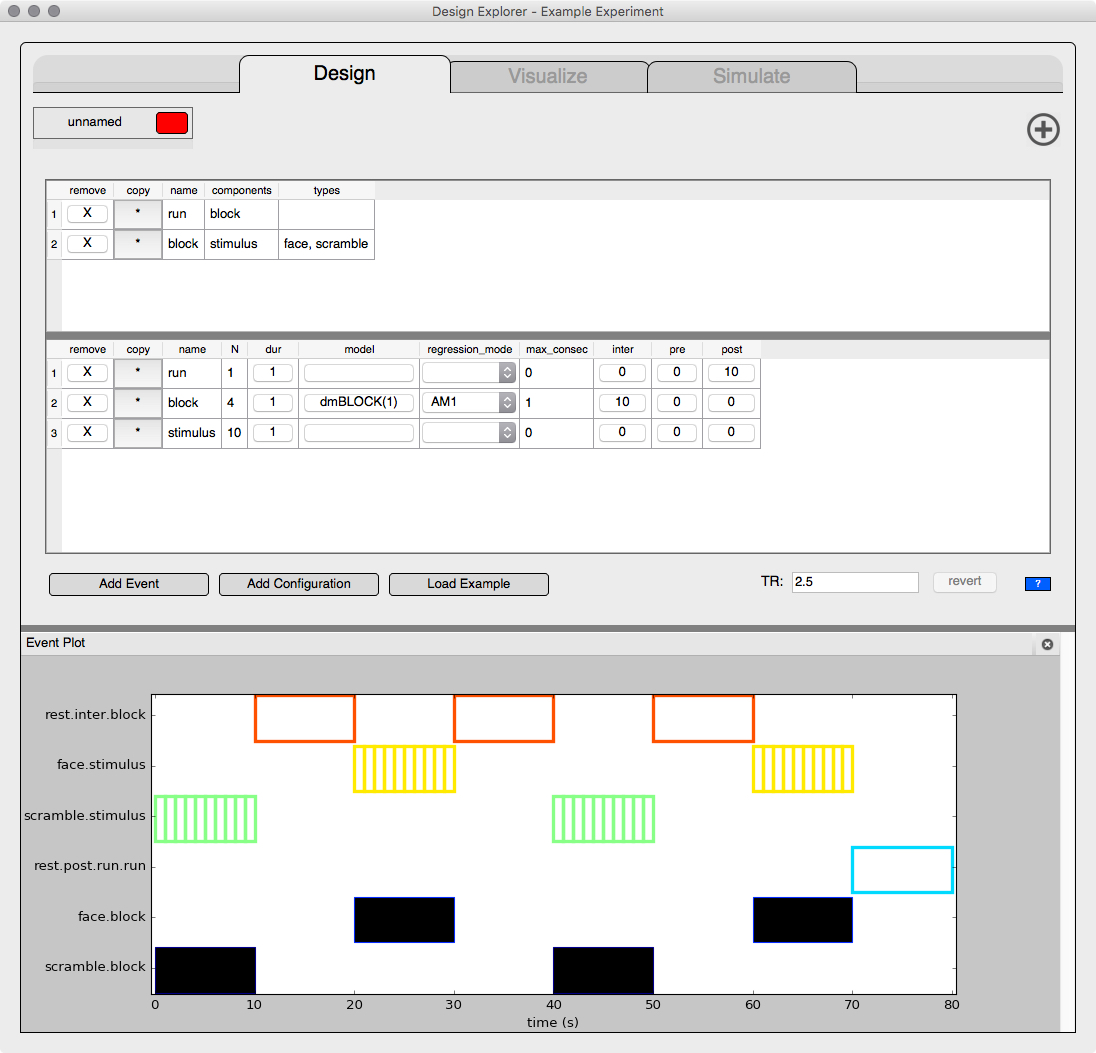
\includegraphics[width=0.75\textwidth,frame]{fig/3_design_full.jpg}
			\caption{Design Tab interface}
			\label{fig:design_over}
		\end{figure}

		\begin{enumerate}
			\item The \hyperref[subsec:event_table]{Event Definition Table} (\textcolor{blue}{\circled{1}})
			\item Add event to the \hyperref[subsec:event_table]{Event Definition Table} (\textcolor{blue}{blue} circle)
			\item The \hyperref[subsec:event_config]{Event Configuration Table} (\textcolor{Purple}{\circled{2}})
			\item Add event to the \hyperref[subsec:event_config]{Event Configuration Table} (\textcolor{Purple}{Purple} circle)
			\item \textbf{TR} entry: Change the repetition time (in seconds)
			\item The \hyperref[subsubsec:revert]{Revert Button}
			\item The \hyperref[subsubsec:hbut]{Help Button} (\hbut{})
			\item The \hyperref[subsec:event_plot]{Event Plot}
		\end{enumerate}

	\subsection{Event Definition Table}
	\label{subsec:event_table}
		The Event Definition Table is where you specify the event hierarchy of the experiment.
		This table has 5 columns:
		\begin{enumerate}
			\item \textbf{remove}

				This column consists of a button that, if clicked, will delete this row from the table.

			\item \textbf{copy}

				This column consists of a button that, if clicked, will copy this row into a new row.

			\item \textbf{name}

				This column consists of a text entry field that will take the user-defined name of an event.
				Event names should be short, but identifiable strings with no spaces.
				Each event row must have a unique name.

			\item \textbf{components}

				This column consists of a text entry field that will take other event names that will be nested within the event defined in the \textbf{name} column.
				These names should also be short strings with no spaces.
				Multiple components should be separated by a comma.
				See \hyperref[subsubsec:def_ex]{below} for examples.

			\item \textbf{types}
		\end{enumerate}

		\subsubsection{Event Definition Examples}
		\label{subsubsec:def_ex}


	\subsection{Event Configuration Table}
	\label{subsec:event_config}

	\subsection{The Event Plot}
	\label{subsec:event_plot}





\section{Visualize Tab}
\label{sec:visualize}
	\subsection{Overview of Interface}
		With a figure, briefly describing the functionality of each button
		\subsubsection{Events}
		\subsubsection{Parameters}
		\subsubsection{Options}
		\subsubsection{Visualizer}
	\subsection{Comparing Variants}

\section{Simulate Tab}
\label{sec:simulate}
	\subsection{Overview of Interface}
	With a figure, briefly describing the functionality of each button
		\subsubsection{Events}
		\subsubsection{Parameters}
		\subsubsection{Options}
		\subsubsection{Visualizer}
		\subsubsection{Simulation}






\end{document}




